\chapter{Introduction to the course. Function classes for optimization.}

\graphicspath{{chapters/01_introduction/figures}}
\begin{abstract}
We summarize first-order and second-order conditions for local minima, 
recall differential notation, discuss error sources in numerical 
differentiation, and collect basic convexity, strong convexity, and 
Lipschitz smoothness facts that will be used throughout the course.
\end{abstract}

\section{Optimization problem}
We will start our course with a study of unconstrained optimization problems 
of the form
\[
  f(x) \rightarrow \min _{x \in \mathbb{R}^{n}} ,
\]
with the practical goal of finding minima. Gradients and Hessians
are denoted by
\[
\nabla f(x)=\begin{pmatrix} \frac{\partial f}{\partial x_1}\\ \vdots\\ 
\frac{\partial f}{\partial x_n} \end{pmatrix} \in \mathbb{R}^{n }, \qquad
\nabla^{2} f(x)=\left\{\frac{\partial^{2} f}{\partial x_{i}\partial x_{j}}
\right\}_{i, j=1}^{n} \in \mathbb{R}^{n \times n} .
\]
\begin{figure}[h]
    \centering
    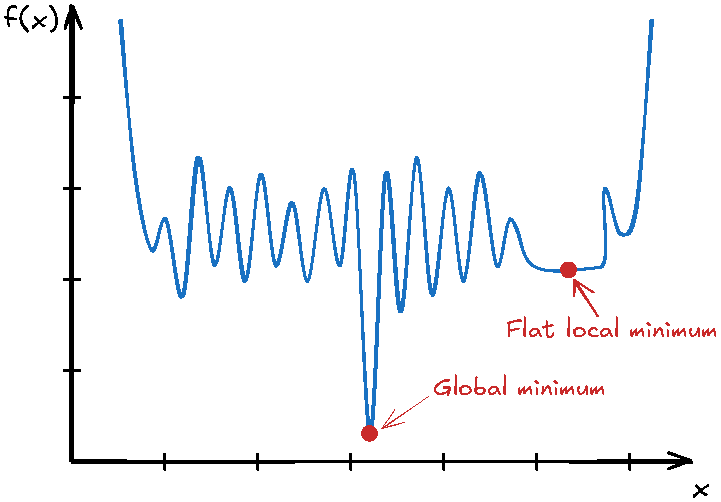
\includegraphics[width=0.6\textwidth]{global_flat.pdf}
   \caption{Rugged nonconvex loss with many minima and a sharp 
   global minimum.}\label{fig:global_flat}
\end{figure}
%\hfill
\noindent Many ML losses are highly nonconvex, with numerous sharp minima 
(see \Cref{fig:global_flat}). The sharp global minimum can make the final 
model sensitive to inputs and noise, while flatter local minima often yield 
more robust solutions even if their objective value is slightly higher. 
In general, finding a good local minimum can be more valuable than finding
the global minimum.
Therefore, our first goal is not necessarily to rush toward the 
global minimum, but to find a good local minimum: this is often easier and 
can lead to better results. We start by reviewing basic optimality 
conditions for local minima.

\hfill
\section{Local optimality conditions}
In many problems, the first step is to write down optimality 
conditions: in simple cases they can lead to a closed-form solution, 
and in iterative algorithms they often serve as stopping criteria.

\begin{definition}[Local minimum]
A point $x$ is a (non-strict) local minimum of $f$ if there exists 
$\varepsilon>0$ such that

\[
  f(y)\ge f(x)\quad \forall y\in O_\varepsilon(x):=\{y:\|y-x\|<\varepsilon\}.
\]

If the inequality is strict for all $y\neq x$ in $O_\varepsilon(x)$, 
then $x$ is a strict local minimum.
\end{definition}


\begin{claim}[Necessary condition of a local minimum]
If $f \in C^{1}$, $x \in \operatorname{int}(\operatorname{dom} f)$, and $x$ is 
a local minimum, then $\nabla f(x)=0$. If in addition $f \in C^{2}$, 
then $\nabla^{2} f(x) \succeq 0$.
\end{claim}
\begin{proof}
Let $d\in\mathbb{R}^n$ be arbitrary and define the one-dimensional function
\[
  \varphi(\alpha)=f(x+\alpha d).
\]
Since $x$ is a local minimum and $x\in \operatorname{int}
(\operatorname{dom} f)$, for sufficiently small $|\alpha|$ we have
$x+\alpha d\in \operatorname{dom} f$ and $\varphi(\alpha)\ge \varphi(0)$, 
so $\alpha=0$ is a local minimum of $\varphi$.
Because $f\in C^1$, we can use Taylor expansion:
\[
\varphi(\alpha) = \varphi(0) + \varphi'(0)\alpha + o(\alpha) \ge \varphi(0) 
\overset{{:\alpha}}{\implies} \varphi'(0)+ o(1) \ge 0 
\overset{\alpha \to 0}{\implies} \varphi'(0) \ge 0
\]
Hence, we get $\varphi'(0) = \nabla f(x)^{\top} d \ge 0 \:\forall d$. This 
means that if we take $d$ and $-d$ equation is only possible if $\nabla f(x) = 0$.
If in addition $f\in C^2$, then for any $d$ we have the second-order 
expansion

\[
  f(x+\alpha d)=f(x)+\alpha\nabla f(x)^\top d
  +\frac{\alpha^2}{2}d^\top\nabla^2 f(x)\,d+o(\alpha^2).
\]

Using $\nabla f(x)=0$ and the same logic as above we can get that 
$d^\top\nabla^2 f(x)\,d\ge 0$ for all $d$, i.e.\ $\nabla^2 f(x)\succeq 0$.
\end{proof}

\textbf{Why just necessary?}
\begin{figure}[h]
  \centering
  \includesvg[width=0.85\textwidth]{why_notsuff}
  \caption{Explanation why $\nabla^2 f\succeq 0$  and $ \nabla f = 0$
  just necessary conditions.}
  \label{fig:why}
\end{figure}

\noindent A stationary point with $\nabla f(x)=0$ can be a local minimum, 
a local maximum, or a saddle point.
The condition $\nabla^2 f(x)\succeq 0$ rules out strict local maxima, 
but still allows saddle points when the Hessian is only 
semidefinite (see \Cref{fig:why}).

\begin{claim}[Sufficient condition of a local minimum]
If $f \in C^{2}$, $x \in \operatorname{int}(\operatorname{dom} f)$, 
$\nabla f(x)=0$, and $\nabla^{2} f(x) \succ 0$, then $x$ is a local minimum.
\end{claim}
\begin{proof}
By the second-order Taylor expansion,
\[
  f(x+h)=f(x)+\nabla f(x)^\top h+\frac{1}{2}h^\top\nabla^2 f(x)\,
  h+o(\|h\|^2).
\]
If $\nabla f(x)=0$ and $\nabla^2 f(x)\succ 0$, then
$h^\top\nabla^2 f(x)\,h>0$ for all $h\ne 0$. Therefore, for sufficiently
small $h\ne 0$ we have $f(x+h)>f(x)$.
\end{proof}

\section{Differentials}

\begin{definition}
The function $f$ is differentiable at $x$ if
\[
f(x+h)-f(x)=\mathrm{d} f(x)[h]+o(\|h\|),
\]
where $\mathrm{d} f(x)$ is a linear operator.
\end{definition}

\begin{definition}
The second differential is
\[
\mathrm{d}^{2} f(x)\left[h_{1}, h_{2}\right]=\mathrm{d}\left(\mathrm{d} 
f(x)\left[h_{1}\right]\right)(x)\left[h_{2}\right].
\]
\end{definition}

\noindent For a scalar function $f:\mathbb{R}^n\to\mathbb{R}$, 
the first differential is the scalar product with the gradient:
\[
  \mathrm{d} f(x)[h]=\nabla f(x)^\top h.
\]
The second differential is a bilinear form linked to the Hessian:
\[
  \mathrm{d}^2 f(x)[h_1,h_2]=h_1^\top \nabla^2 f(x)\,h_2.
\]

\begin{example}[A worked example: $f(x)=\frac{1}{3}\|x\|_2^3$]
Let $f(x)=\frac{1}{3}\|x\|_2^3=\frac{1}{3}(x^\top x)^{3/2}$. For $x\neq 0$,
\[
  \nabla f(x)=\|x\|_2\,x,
  \qquad
  \nabla^2 f(x)=\frac{1}{\|x\|_2}xx^\top+\|x\|_2 I.
\]
(At $x=0$ one can take $\nabla f(0)=0$ and $\nabla^2 f(0)=0$.)
\end{example}

\section{Error analysis and machine precision}

In the algorithms covered in this book we will use only real numbers. However, modern
computes are not able to store and work with general real numbers. Instead, they
work only with a finite subset known floating-point numbers. It means that
in computations we will get just approximations of these numbers. So, we want 
to do this approximations as close to theoretical one as possible.
In floating-point arithmetic a real number is stored  in the form 
$\mathrm{fl}(x)=sM2^E$. Machine precision $\varepsilon_{m}$ 
bounds the relative representation error:
\[
\left|\frac{\mathrm{fl}(x)-x}{x}\right| \leq \varepsilon_{m}\qquad (x\neq 0).
\]
Typical values:
\[
\begin{array}{c|c}
\text { bits } & \varepsilon_{m} \\
\hline
64 & 10^{-16} \\
32 & 10^{-7} \\
16 & 10^{-3}
\end{array}
\]
\begin{figure}[h]
  \centering
  \IfFileExists{chapters/01_introduction/figures/finite_diff_tradeoff.pdf}{%
    \includegraphics[width=0.6\textwidth]{finite_diff_tradeoff.pdf}%
  }{%
    \fbox{\parbox{0.7\textwidth}{\centering
      TODO figure: \texttt{finite\_diff\_tradeoff.pdf}.\\
      Plot $\log_{10}(\text{error})$ vs.\ $\log_{10}(\varepsilon)$ showing\\
      truncation ($\sim\varepsilon$), roundoff
      ($\sim\varepsilon_m/\varepsilon$), and
      $\varepsilon_{\text{opt}}\approx\sqrt{\varepsilon_m}$.}}%
  }
  \caption{Truncation--roundoff trade-off in finite-difference differentiation.}
  \label{fig:finite-diff-tradeoff}
\end{figure}
\section{ Classes of functions}
Unfortunately, the use of Taylor expansion is restricted by the fact that 
it is useful only in the vicinity of the point. So, in order to prove 
convergence of optimization algorithms we will need to introduce common
classes of functions which will work globally rather than locally.
\subsection{Convexity and strong convexity}

\begin{definition}[Convex function]
A function $f$ is convex if for all $x,y$ and $\alpha\in[0,1]$,
\[
  f(\alpha x+(1-\alpha)y)\le \alpha f(x)+(1-\alpha)f(y).
\]
It is strictly convex if the inequality is strict for $x\ne y$ and 
$\alpha\in(0,1)$.
\end{definition}

\begin{figure}[h]
  \centering
  \IfFileExists{chapters/01_introduction/figures/convex_chord.pdf}{%
    \includegraphics[width=0.5\textwidth]{convex_chord.pdf}%
  }{%
    \fbox{\parbox{0.7\textwidth}{\centering
      TODO figure: \texttt{convex\_chord.pdf}.\\
      Draw a convex curve with the chord between $(x,f(x))$ and $(y,f(y))$\\
      lying above the graph.}}%
  }
  \caption{Geometric meaning of convexity: chords lie above the graph.}
  \label{fig:convex-chord}
\end{figure}
\noindent A function is concave if $-f$ is convex (strictly concave if
$-f$ is strictly convex).

\begin{claim}[Differential criteria of convexity]
Let $f \in C^{1}$. Then $f$ is convex if and only if for all $x, y$,
\[
f(y) \geq f(x)+\nabla f(x)^{\top}(y-x) .
\]
If $f \in C^{2}$, then $f$ is convex if and only if $\nabla^{2} f(x) 
\succeq 0$ for all $x$.
\end{claim}

\begin{definition}
The function $f$ is $\mu$-strongly convex if for all $x$ the function 
$f(x)-\frac{\mu}{2}\|x\|^{2}$ is convex.
\end{definition}

\begin{claim}[Differential criteria of strong convexity]
If $f \in C^{1}$, then $f$ is $\mu$-strongly convex if and only if for 
all $x, y$,
\[
f(y) \geq f(x)+\nabla f(x)^{\top}(y-x)+\frac{\mu}{2}\|x-y\|^{2} .
\]
If $f \in C^{2}$, then $f$ is $\mu$-strongly convex if and only if
$\nabla^{2} f(x) \succeq \mu I \succ 0$ for all $x$.
\end{claim}

\subsection{Lipschitz classes}

\begin{definition}
The function $f$ belongs to the Lipschitz class $C_{L}^{k, m}$ if (i) 
$f \in C^{k}$, (ii) $m \leq k$, and (iii)
\[
\left\|\nabla^{m} f(x)-\nabla^{m} f(y)\right\| \leq L\|x-y\|
\quad \forall x, y .
\]
\end{definition}
\begin{figure}[h]
  \centering
  \IfFileExists{chapters/01_introduction/figures/l_smooth_bounds.pdf}{%
    \includegraphics[width=0.55\textwidth]{l_smooth_bounds.pdf}%
  }{%
    \fbox{\parbox{0.7\textwidth}{\centering
      TODO figure: \texttt{l\_smooth\_bounds.pdf}.\\
      Sketch tangent at $y$ and the upper/lower quadratic envelopes from\\
      the $C_L^{1,1}$ inequalities.}}%
  }
  \caption{For $C_L^{1,1}$ functions, the graph is sandwiched between two
    quadratic models around $y$.}
  \label{fig:l-smooth-bounds}
\end{figure}

\paragraph{Examples.}
\begin{enumerate}
\item If $f \in C_{L}^{0,0}$, then $|f(x)-f(y)| \leq L\|x-y\|$ for all $x, y$,
  equivalently
\[
f(y)-L\|x-y\| \leq f(x) \leq f(y)+L\|x-y\| .
\]
\item If $f \in C_{L}^{1,1}$, then
\[
f(x) \geq f(y)+\nabla f(y)^{\top}(x-y)-\frac{L}{2}\|x-y\|^{2},
\]
\[
f(x) \leq f(y)+\nabla f(y)^{\top}(x-y)+\frac{L}{2}\|x-y\|^{2}.
\]
\end{enumerate}

\begin{claim}
$f \in C_{L}^{k, m-1} \iff \|\nabla^{m} f(x)\| \leq L$.
\end{claim}

\section{Finite differentiation}

We approximate directional derivatives $g:=\nabla f(x)^{\top} d$ with
stepsize $\varepsilon$ in floating-point arithmetic. We write
$\mathrm{fl}(\cdot)$ for computed quantities and use the model
\[
  |\mathrm{fl}(z)-z| \leq |z|\,\varepsilon_{m}.
\]

\paragraph{Forward difference.}
The Taylor expansion gives
\[
  f(x+\varepsilon d)=f(x)+g\,\varepsilon+O(\varepsilon^{2}),
\]
so
\[
  g=\frac{f(x+\varepsilon d)-f(x)}{\varepsilon}+O(\varepsilon).
\]
Define the computed estimator
\[
  \widehat g_{\mathrm{fd}}(\varepsilon)=
  \mathrm{fl}\!\left(\frac{f(x+\varepsilon d)-f(x)}{\varepsilon}\right).
\]
Then
\[
  |g-\widehat g_{\mathrm{fd}}(\varepsilon)|
  \le |g-\tfrac{f(x+\varepsilon d)-f(x)}{\varepsilon}|
  +\left|\tfrac{f(x+\varepsilon d)-f(x)}{\varepsilon}
  -\widehat g_{\mathrm{fd}}(\varepsilon)\right|.
\]
Assume $|f(\cdot)|\le L_0$ in a neighborhood of $x$, and the truncation
error satisfies
\[
  \left|g-\tfrac{f(x+\varepsilon d)-f(x)}{\varepsilon}\right|
  \le L_2\,\varepsilon.
\]
Then the roundoff term is bounded by
\[
  \left|\tfrac{f(x+\varepsilon d)-f(x)}{\varepsilon}
  -\widehat g_{\mathrm{fd}}(\varepsilon)\right|
  \le \varepsilon_m\,\tfrac{|f(x+\varepsilon d)|+|f(x)|}{\varepsilon}
  \le \tfrac{2L_0\,\varepsilon_m}{\varepsilon}.
\]
Therefore
\[
  |g-\widehat g_{\mathrm{fd}}(\varepsilon)|
  \le L_2\,\varepsilon+\tfrac{2L_0\,\varepsilon_m}{\varepsilon}.
\]
This shows that taking $\varepsilon$ too small increases the error due to
roundoff. Minimizing the bound gives
\[
  \varepsilon_{\mathrm{opt}}=
  \sqrt{\tfrac{2L_0\,\varepsilon_m}{L_2}}
  \approx \sqrt{\varepsilon_m}.
\]

\paragraph{Central difference.}
Using the expansions
\[
  f(x+\varepsilon d)=f(x)+g\,\varepsilon
  +\tfrac{1}{2}d^\top\nabla^2 f(x)d\,\varepsilon^2+O(\varepsilon^3),
\]
\[
  f(x-\varepsilon d)=f(x)-g\,\varepsilon
  +\tfrac{1}{2}d^\top\nabla^2 f(x)d\,\varepsilon^2+O(\varepsilon^3),
\]
we get
\[
  g=\frac{f(x+\varepsilon d)-f(x-\varepsilon d)}{2\varepsilon}
  +O(\varepsilon^2).
\]
With the computed estimator
\[
  \widehat g_{\mathrm{cd}}(\varepsilon)=
  \mathrm{fl}\!\left(\frac{f(x+\varepsilon d)-f(x-\varepsilon d)}
  {2\varepsilon}\right),
\]
and assuming $|f(\cdot)|\le L_0$ in the neighborhood of $x$ and 
a truncation bound $|O(\varepsilon^2)|\le L_3\varepsilon^2$, we obtain
\[
  |g-\widehat g_{\mathrm{cd}}(\varepsilon)|
  \le L_3\,\varepsilon^2+\tfrac{L_0\,\varepsilon_m}{\varepsilon}.
\]
Minimizing yields
\[
  \varepsilon_{\mathrm{opt}}=
  \sqrt[3]{\tfrac{L_0\,\varepsilon_m}{2L_3}}
  \approx \sqrt[3]{\varepsilon_m}.
\]

\paragraph{Complex step.}
If $f$ is an analytic function, then
\[
  f(x+i\varepsilon d)=f(x)+i g\,\varepsilon+O(\varepsilon^2)+iO(\varepsilon^3),
\]
so
\[
  g=\frac{\operatorname{Im} f(x+i\varepsilon d)}{\varepsilon}
  +O(\varepsilon^2).
\]
The reason why previous schemes were unstable is $a - b $, 
where $a \approx b$, which is very unstable in floating-point. 
This method avoids subtracting close numbers, so we can take
$\varepsilon_{\mathrm{opt}}=\varepsilon_m$.
\paragraph{Gradient checking (practical note).}
Finite differences are a simple sanity check for analytical gradients in
code: sample a random direction $d$ and compare $\nabla f(x)^\top d$
with a difference quotient using the recommended $\varepsilon$ scales above.
